\subsection{Standardisation} \label{subsec: Standardisation}
Type Ia Supernovae (SNe Ia) are standardisable candles, which means that upon observation of a SN Ia, the observed brightness follows a predictable evolution\parencite{martin_o_2024,rigault_strong_2020}. With corrections for the stretch and colour of the SN, the light curve can be standardised which corrects the observed light curve to find the intrinsic luminosity of the SNe Ia. The corrections for the light curves can be found in equation \ref{Eq: The Tripp equation} which accounts for the colour and stretch of the supernovae to determine the distance modulus (\(\mu_{obs}\)) \parencite{tripp_two-parameter_1998}. Using this distance modulus you can then derive distances to the Supernovae. 

\begin{equation}
    \mu_{obs} = m^*_B-M_B + \alpha x_1-\beta c
    \label{Eq: The Tripp equation}
\end{equation}

In equation \ref{Eq: The Tripp equation} the distance modulus is the difference between the apparent magnitude, \(m^*_B\), of the supernova and the absolute magnitude, \(M_B\) of the supernova. The remaining parameters are the stretch \(x_1\) and the colour \(c\) where \(\alpha\) and \(\beta\) are the stretch and colour coefficients where \(\alpha\) falls between 0.14 and 0.15 and \(\beta\) is between 2.9 and 3.5 \parencite{brout_pantheon_2022, martin_o_2024}. 

The stretch parameter is the parameter that corrects for the width of the light curve due to different distributions and masses of \ce{^{56}Ni} in the ejecta of the supernova \parencite{deckers_constraining_2022}. The colour is corrected due to the intrinsic components of the supernova and the surrounding environment such as dust, which can cause a redshift of the light, altering the shape of the light curve \parencite{kelsey_concerning_2022}. \(m^*_B\) is the apparent magnitude of the SNe Ia which is how bright the object appears from Earth and \(M_B\) is the absolute magnitude of the SNe Ia which is how bright the SNe Ia is from 10 parsecs away. 

Using the resulting \(\mu_{obs}\) from equation \ref{Eq: The Tripp equation}, you can acquire the luminosity distance \(d_L\) to the object using equation \ref{Eq: luminosity distance equation from distance modulus}, noting that the coefficient 10 is in units of parsecs \parencite{brout_pantheon_2022}. 

\begin{equation}
    d_L = 10 (10^{\mu/5})\
    \label{Eq: luminosity distance equation from distance modulus}
\end{equation}

From this equation, the luminosity distance can then be used to calculate cosmological parameters such as the density parameters for matter and radiation \(\Omega_m\) and \(\Omega_r\) and the equation of state parameter that describes how the density of matter, radiation and dark energy change in time \(w_{m}, w_{r}, w_{\Lambda}\) \parencite{brout_pantheon_2022}. Cosmological quantities are important, as they represent the contents of the Universe and thus be used to determine properties of the Universe. Standardisation of the supernovae and accounting for the different stretches and colours that are observed in the light curves results in more accurate distance calculations and better calculations of the cosmological parameters. 

The standardisation of SNe Ia light curves are not perfect, \textcite{brout_pantheon_2022,martin_o_2024,wiseman_further_2023,rigault_strong_2020} all show how the Tripp equation still leaves residual scatter of the distance modulus, which can be seen in Figure \ref{fig: Martin et al., 2024 Hubble Residuals as a function of galaxy stellar mass}. Research continues to determine how to improve standardisation methods that result in cosmological parameters that better represent the observed properties of the Universe. The Hubble residual is the measure of scatter in the calculation of the distance modulus, it's determined by the subtraction of the distance modulus calculated from a specific cosmology, \(\mu_{cos}\), from the result of equation \ref{Eq: The Tripp equation}, seen in equation \ref{Eq: Hubble residual equation}. It has been found that the scatter after corrections using the Tripp equation is reduced to 0.15 magnitude, leading to the conclusion that further corrections based on different properties are needed to standardise these light curves \parencite{brout_pantheon_2022,kelsey_concerning_2022, martin_o_2024}.

\begin{equation}
    \Delta\mu = \mu_{obs} - \mu_{cos}\
    \label{Eq: Hubble residual equation}
\end{equation}

\begin{figure}[htbp]
    \centering
    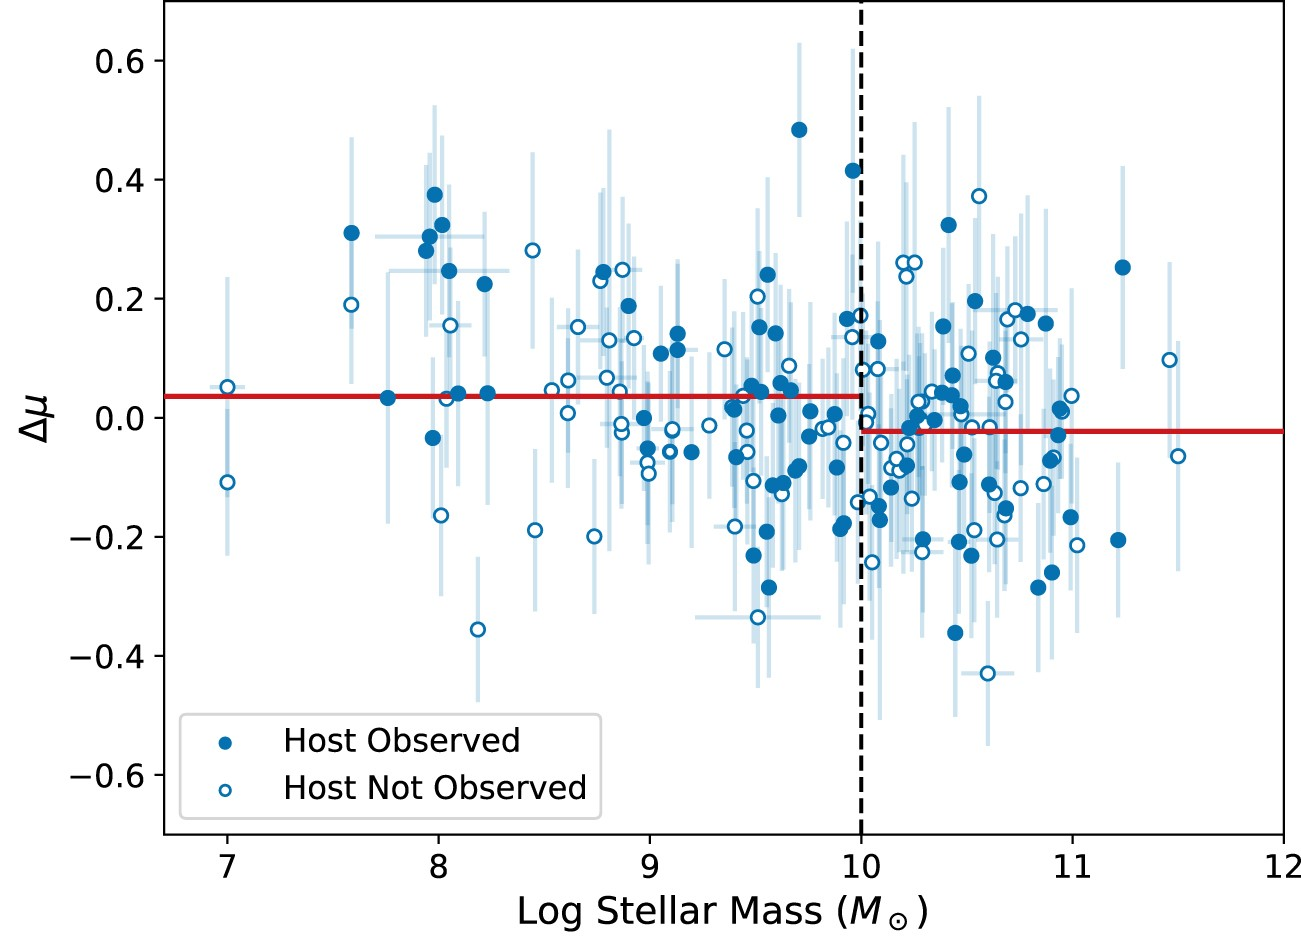
\includegraphics[width=0.8\linewidth]{graphics/SNIa_Physics_and_Progenitor_Channels/Hubble_residuals_Martin_2024.png}
    \caption{A figure taken from \textcite{martin_o_2024} that shows the scatter in Hubble residuals using 179 SNe Ia from the Foundation Survey dataset that is used in \textcite{martin_o_2024}'s analysis as a function of the host galaxy mass. The average Hubble residual is a step function at a host galaxy stellar mass of \(10\textup{M}_\odot\).}
    \label{fig: Martin et al., 2024 Hubble Residuals as a function of galaxy stellar mass}
\end{figure} 
    
A contentious correction that is made after the corrections made in equation \ref{Eq: The Tripp equation} to the SNe Ia light curves, is that of the host galaxy mass step\parencite{kelly_hubble_2010,sullivan_dependence_2010, lampeitl_effect_2010}. This remaining correlation showed that SNe Ia are 10 per cent brighter in more massive host galaxies, which lead to a noticeable difference in the equation of state parameter for dark energy (\(w_{\Lambda}\)). \textcite{kelly_hubble_2010}, who found that SNe Ia in more massive host galaxies were\(\simeq 0.1\) mag brighter than SNe Ia in less massive host galaxies, used 70 SNe Ia from the Sloan Digital Sky Survey with a redshift range \(0.015<z<0.08\) and determined that when using \(\mu_{obs}\) from 30 SNe Ia with host galaxies that have a stellar mass less than \(10^{10.8}\textup{M}_\odot\) the equation of state parameter is  \(w_{\Lambda} = -0.78^{+0.152}_{-0.108}\) whereas for 30 SNe Ia with host galaxies with a stellar mass greater than \(10^{10.8}\textup{M}_\odot\),\(w_{\Lambda} = -1.03^{+0.217}_{-0.143}\).

For the standard \(\Lambda\)CDM model of the Universe, the density of dark energy is taken as constant which implies an equation of state parameter \(w_{\Lambda}=-1\). And as can be seen in \textcite{kelly_hubble_2010}, using SNe Ia that are in less massive galaxies don't reflect the \(w=-1\) that is accepted in the modern model of the Universe. The error goes beyond the uncertainty of the determination of \(w_{\Lambda}\), showing that there is a systematic error in the standardisation of SNe Ia samples that are used in cosmology. This finding by \textcite{kelly_hubble_2010} was corroborated by \textcite{lampeitl_effect_2010} who used 361 SNe Ia from the SDSS-II Supernova Survey and limited the redshifts of the sample to \(z<0.21\). \textcite{lampeitl_effect_2010} found the more massive and lesser star formation rate (SFR) galaxies, hosted SNe Ia that were \(\simeq 0.1\) mag brighter than SNe Ia that were in galaxies of lower stellar masses. Finally, \textcite{sullivan_dependence_2010} using 195 SNe Ia from the Supernova Legacy Survey within redshift \(z <0.85\) also independently found that SNe Ia in higher mass host galaxies are 0.06–0.09 mag brighter than SNe Ia in galaxies with lower stellar mass. 

Although older, \textcite{kelly_hubble_2010,sullivan_dependence_2010, lampeitl_effect_2010} independently found the correlation of Hubble residuals with the stellar mass of the supernovas host galaxy and provided the initial mass step correction to further standardise supernova light curves. \textcite{kelly_hubble_2010,sullivan_dependence_2010, lampeitl_effect_2010} also demonstrates how the mass step is found across three different surveys and a redshift up to 0.85. Showing that the mass step correction is applicable systematically in the light curve measurements of SNe Ia used as standardisable candles in cosmology, although \textcite{kelly_hubble_2010,sullivan_dependence_2010, lampeitl_effect_2010} originally found and corrected for the mass step, the physical mechanics of why this difference in brightness is observed across more massive galaxies is not known. 

\subsection{Progenitor Channels} \label{subsec: Progenitor Channels}
It is accepted that the star that undergoes a supernova, producing the characteristic SNe Ia light curve is a carbon-oxygen (C-O) white dwarf \parencite{hoyle_nucleosynthesis_1960}. But white dwarfs don't undergo a supernova during their evolution, thus requiring other progenitor channels to be explored\parencite{antonini_evolution_2026}. The two popular progenitor channels for SNe Ia are the single degenerate scenario (SD) and the double degenerate scenario (DD). SD proposes that before an SN Ia event occurs, the system that was there before consisted of a C-O white dwarf that was accreting material from a non-degenerate companion star in a binary orbit\parencite{whelan_binaries_1973}. Whilst the DD scenario presents the idea of a merger between two degenerate stars such as two C-O white dwarfs and could also result in a supernova\parencite{iben_supernovae_1984}. 

The SD and DD progenitor models have been popular for decades and with recent research indicating that there is more nuance to these two progenitor channels that can cause the variety of the light curves observed by astronomers. \textcite{deckers_constraining_2022} study shows that out of 115 SNe Ia events that were detected by the Zwicky Transient Facility (ZTF), 67 per cent of the observed supernova light curves could effectively be recreated by the TURTLS model where the luminosity of the explosions are a direct result of Chandrasekhar-mass explosions with extended distributions and masses of 0.4 to 0.6 \(\textup{M}_\odot\) of \ce{^{56}Ni}. \textcite{deckers_constraining_2022} shows that over two thirds of SNe Ia could be resulting from Chandrasekhar mass C-O white dwarf explosions, whilst also demonstrating that 11 per cent of the SNe Ia light curves in the sample aren't reproduced from Chandrasekhar mass explosions and 19 per cent of the sample cannot be constrained using the varied masses and distributions of \ce{^{56}Ni}.   

\textcite{deckers_constraining_2022} also demonstrates a method to determine flux excesses in six light curves of the SNe Ia in the sample, \textcite{deckers_constraining_2022} finds that these flux excesses are generally well produced by the non degenerate companion interaction models as well as the \ce{^{56}Ni} clumping models that also produced the light curves of the 67 per cent of the SNe Ia. Due to the limited sample size \textcite{deckers_constraining_2022} concludes that SNe Ia likely have numerous pathways to explosion hence the varied observed light curves, but it appears that those 67 per cent can be modelled through the SD scenario. \textcite{deckers_constraining_2022} urges more high cadence UV and NUV surveys with spectroscopic follow up be done to conclude with more confidence the explosion scenario of SNe Ia. 

In a similar vein to \textcite{deckers_constraining_2022}, \textcite{burke_early_2022} shows that using a model that used a template light curve of a SN Ia from SiFTO with a companion shock-heating component component on a sample of nine SNe Ia that have light curve data 16 days before the epoch of peak flux, are well fit by non-degenerate companion interaction with the ejecta. These fits support the SD scenario interpretation. \textcite{burke_early_2022} suggests that the ejecta from the mass accreting white dwarf, shock heats the surface of the non-degenerate companion star which produces the flux excess in the light curves. This corroborates with the findings of the six early excess (EEx) SNe Ia in \textcite{deckers_constraining_2022} which reported non-degenerate companion interactions effectively modelled the observed light curves. 

Interestingly \textcite{burke_early_2022} also reported that eight of the nine SNe Ia were near-UV to Blue in colour (i.e. SNe Ia that have negative colour parameter $c$), although \textcite{deckers_constraining_2022} only reports three of the six having blue colour whilst the other three were red colour. This observed difference in colour is not reconciled through cross examination of either study. Both studies are still limited to small sample sizes which makes it difficult to make broader conclusions about the cause of the flux excesses and thus difficult to constrain the possible progenitor channels for these SNe Ia. Both papers conclude that high cadence near-UV surveys that detect more SNe Ia early on will help in our understanding of these flux excesses in the light curves. 

Although light curve fitting and modelling has shown results in determining the possible progenitors systems of SNe Ia, there have been numerous studies on the correlations of SNe Ia light and the Host galaxy properties. \textcite{kelsey_concerning_2022} finds through the analysis of 675 photometrically classified SNe Ia from the Dark Energy Survey 5-year sample, that blue SNe Ia are found in host galaxies that have lower stellar mass with higher star formation rates and are more blue in colour. \textcite{kelsey_concerning_2022} makes the argument that the stars in these hosts are younger populations that are producing the more blue colours. 

Although an older study, \textcite{anderson_environments_2015} finds a similar trend with SNe Ia light tracing out the blue light from host galaxies using pixel statistics method. \textcite{anderson_environments_2015} asserts that because the light from SNe Ia traces out the bluer region of host galaxies with lower SFR that progenitors systems that are less than 100 Myr old are extremely rare or do not exist. \textcite{kelsey_concerning_2022} also finds this 'colour gradient' where star formation begins closer to the centre of the host galaxy and eventually spreading to the outskirts of the host. But \textcite{anderson_environments_2015} using the pixel method found that the more 'local' lower star formation rates host the bluer SNe Ia, leading to older progenitor systems producing SNe Ia. \textcite{kelsey_concerning_2022} finds that the colour of the SNe Ia as a function of the local host galaxy colour is more blue in more locally bluer host environments, both these findings would suggest that the progenitor systems of SNe Ia are old and happening in bluer environments.   

\subsection{Early Flux Excess} \label{subsec: Early Flux Excess}
Early flux excess in the light curves of SNe Ia are seen as bumps in the light curve before the flux of the SNe Ia has reached its peak. In 2012 a SN Ia was observed and the analysis of the light curve by \textcite{marion_sn2012cg_2016} showed an EEx flux in the V, B and U band photometry. This was the first analysis of a 'normal' SNe Ia that had an EEx flux and the conclusion drawn was that the progenitor system likely was a non-degenerate companion, that was shock heated and was lucky enough to have the right viewing angle so that the excess could be observed. 

\textcite{burke_early_2022} uses data which was obtained from high cadence follow up observations using Las Cumbres Observatory and Swift, found 9 SNe Ia that had good early light curve data. \textcite{burke_early_2022} found that the light curves were best explained via the shock heating of a non-degenerate companion where a C-O white dwarf was accreting mass from this companion and upon explosion, had ejecta interactions with the companion that results in the companion, at the right angle, emitting a near-U-V blue excess. This again corroborates with the discovery \textcite{marion_sn2012cg_2016} proposes that companion interactions with a non-degenerate star is the physical cause of the EEx observed.

Referring back to \textcite{deckers_constraining_2022} who had a sample size of 6 EEx SNe Ia, found that the EEx colour and the lifetime of the flux excess is consistent with their modelling of both companion and circumstellar medium (CSM) interaction as well as \ce{^{56}Ni} clumping in the outer ejecta of the white dwarf. \textcite{deckers_constraining_2022} argues that the EEx flux in SNe Ia is heterogeneous and can be caused by multiple different progenitors. \textcite{deckers_constraining_2022} is to contrast the previous studies as they conclude, that to be more definitive regarding the mechanisms behind the EEx in flux, one day cadence surveys will enable fast spectroscopic follow up which will grant the ability to make more confident conclusions about the physics of the EEx.

\textcite{lim_early_2023} is a case study on SN 2021hpr which exhibits the EEx in it's flux, similar to \textcite{marion_sn2012cg_2016} and \textcite{burke_early_2022}, the shock heating emission of the companion star for the white dwarf most suitably models the light curves of SN 2021hpr across the B, V, R and I bands from the Intensive Monitoring of Nearby Galaxies Survey which can be seen in Figure \ref{fig: Lim et al., 2023 the light curve of SN2021hyp}. Although the light curve fit well with a non degenerate companion model, \textcite{lim_early_2023} could not find evidence of any stripped mass of the companion that would've been expected following the explosion of the companion using spectroscopic follow-up. \textcite{lim_early_2023} also acknowledge that they did not assess the viability of other models that could cause the excess, such as a double detonation model or disk originated matter models.

\begin{figure}[htbp]
    \centering
    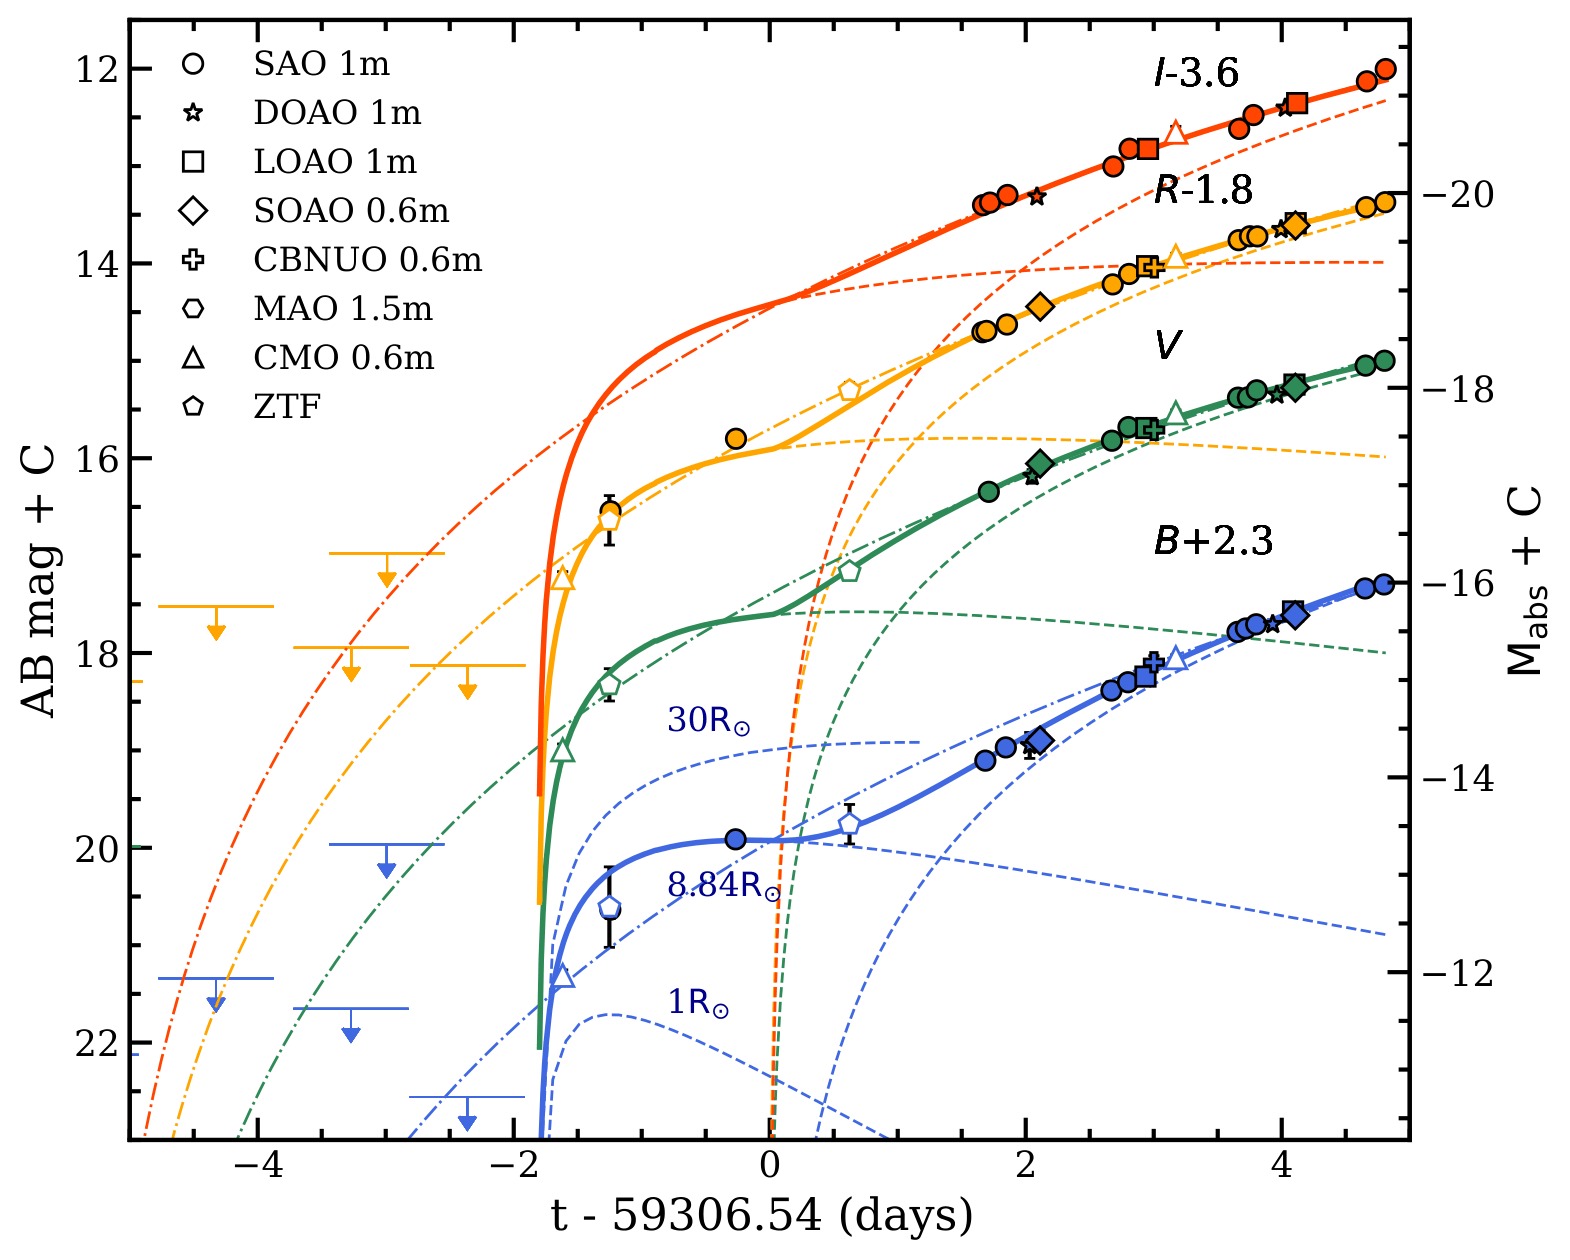
\includegraphics[width=0.8\linewidth]{graphics/SNIa_Physics_and_Progenitor_Channels/lim_2021_hpr_supernova_lightcurve.png}
    \caption{The light curves of SN2021hpr in magnitude space taken from \textcite{lim_early_2023}. The points are the observations, the dashed-dotted line is the light curve modelled by the simple power law model and the dashed lines are modelled light curves from \textcite{kasen_seeing_2010} which include the emission of light from the shock heating of a companion star. Finally, the solid lines are the two models combined and can be seen to line up well with the observations.}
    \label{fig: Lim et al., 2023 the light curve of SN2021hyp}
\end{figure}
 
 \textcite{lim_early_2023} shows that the light curve deviates from a simple power law model as well as the companion model from \textcite{kasen_seeing_2010} and has a bump across all bands which can be seen in Figure \ref{fig: Lim et al., 2023 the light curve of SN2021hyp}. But the combination of both the power law and the \textcite{kasen_seeing_2010} companion models produce a curve that fits the observations. 

The method used to detect the EEx fluxes in the SNe Ia data can vary, in \textcite{deckers_constraining_2022} they use the residuals in the light curves that are found by subtracting the modelled light curve generated using the TURTLS model from the observed light curve. If a positive residual is found in the light curve within the calculated 6 days after the explosion epoch \textcite{deckers_constraining_2022} classify that SNe Ia light curve as an EEx SNe Ia. 

In \textcite{burke_early_2022} the EEx flux SNe Ia are identified in a similar way to what was done in \textcite{lim_early_2023}, as \textcite{burke_early_2022} uses the same companion shock cooling models present in \textcite{lim_early_2023} from \textcite{kasen_seeing_2010}. \textcite{burke_early_2022} stipulates that they classify SNe Ia as EEx SNe Ia if there is data available within five days of the first detection, the best fit viewing angle is less than 90 degrees and the residuals in the g band show a systematic decreasing from the earliest epochs to then matching the modelled light curve. Finally in \textcite{marion_sn2012cg_2016} the EEx flux SNe Ia was detected through the comparison of the observed light curve to the fitted power model light curve where the observed data had to be three times the measurement uncertainty. 